\documentclass[11pt]{beamer}
\usepackage[utf8]{inputenc}
\usepackage[T1]{fontenc}
\usepackage{lmodern}
\usepackage[english]{babel}
\usepackage{amsmath}
\usepackage{amsfonts}
\usepackage{amssymb}
\usepackage{graphicx}
\usetheme{AnnArbor}
\begin{document}
	\author[Soham, Sukhmani, Tarun, Ali]{Soham Sarfare \and Sukhmani Arora \and Tarun Tirupati \and Ali Saeed}
	\title[First Order Model]{ RetinaFace: Single-stage Dense Face Localisation in the Wild}
	\subtitle{Application of Data Science - Project Proposal Presentation Group F}
	%\logo{\includegraphics[height=1.0cm]{logo.png}}
	\institute[]{Faculty of Computing \\ Macquarie University}
	%\date{}
	%\subject{}
	%\setbeamercovered{transparent}
	%\setbeamertemplate{navigation symbols}{}
	\begin{frame}[plain]
		\maketitle
	\end{frame}
	\begin{frame}
		\frametitle{Introduction}
		Name of the Paper: RetinaFace: Single-stage Dense Face Localisation in the Wild\\
		Authors: Jiankang Deng, Jia Guo, Yuxiang Zhou, Jinke Yu, Irene Kotsia, Stefanos Zafeiriou
		\begin{itemize}
			\item This paper tries to overcome the challenges faced in face detection, accurate face localisation.
			\item The paper was published in the IEEE Conference for Computer Vision and Pattern Recognition which has a A1 rating according to Qualis. 
			\item So far, we have managed to run the code on colab and achieved in getting accurate results which are similar to the results stated by authors, along with getting the similar precision-recall graphs.
			\item At the moment , we are focussing on constructing new dataset which will be a compilation of images with respective coordinates and measurements.
			
		\end{itemize}
	\end{frame}
\begin{frame}
	\frametitle{Original Data}
	Outputs produced by the code are evaluted according to the steps provided at http://shuoyang1213.me/WIDERFACE/
	\begin{figure}
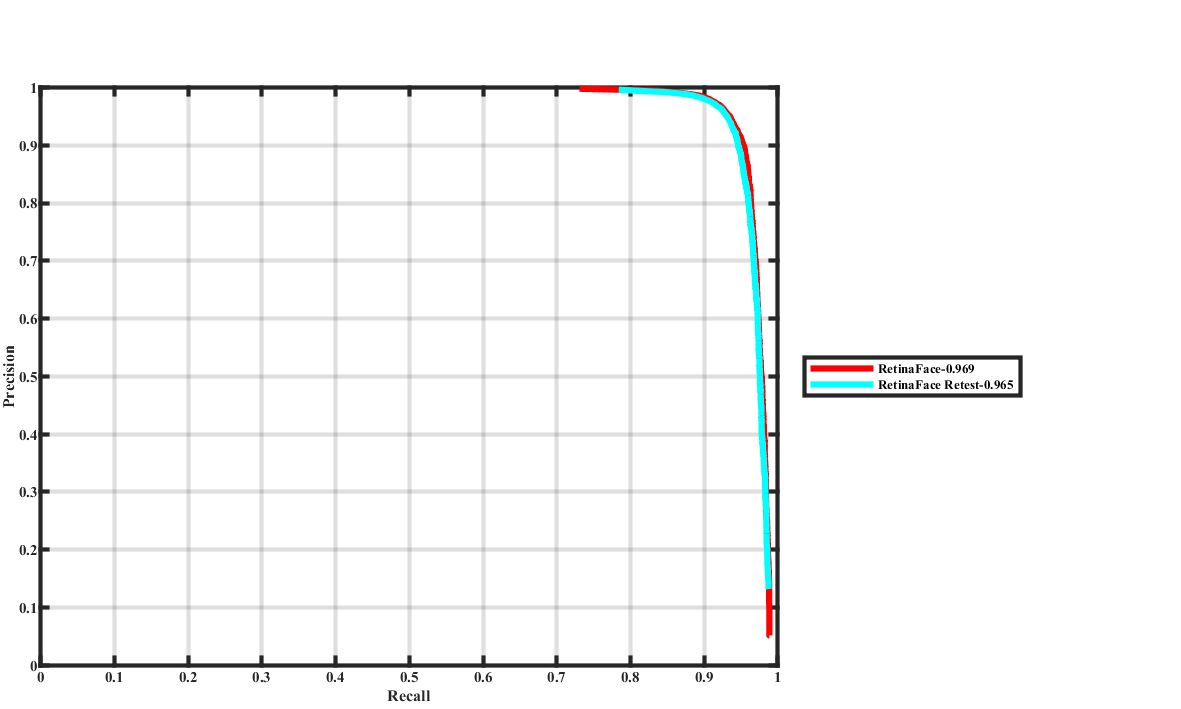
\includegraphics[width=0.75\linewidth]{wider_pr_cruve_int_easy_val.png}
	\caption{Easy Val}
	\end{figure}
	
\end{frame}
\begin{frame}
	\frametitle{Original Data}
	\begin{figure}
		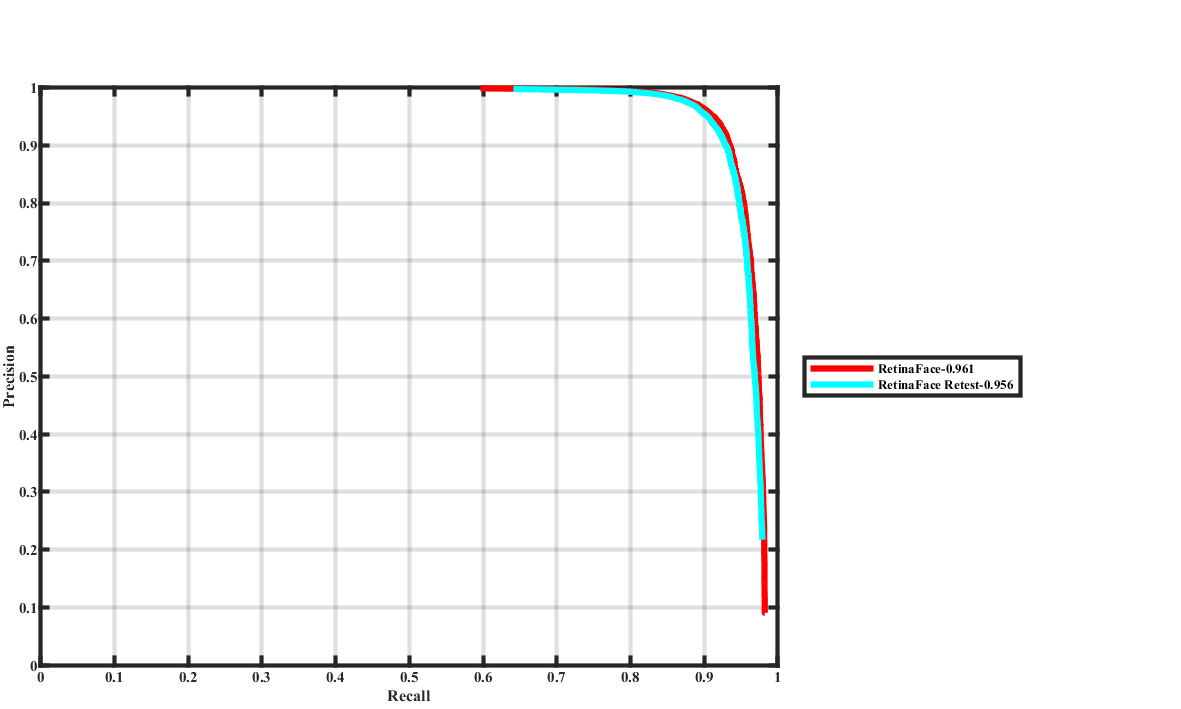
\includegraphics[width=0.75\linewidth]{wider_pr_cruve_int_medium_val.png}
		\caption{Medium Val}
	\end{figure}
	
\end{frame}
\begin{frame}
	\frametitle{Original Data}
	\begin{figure}
		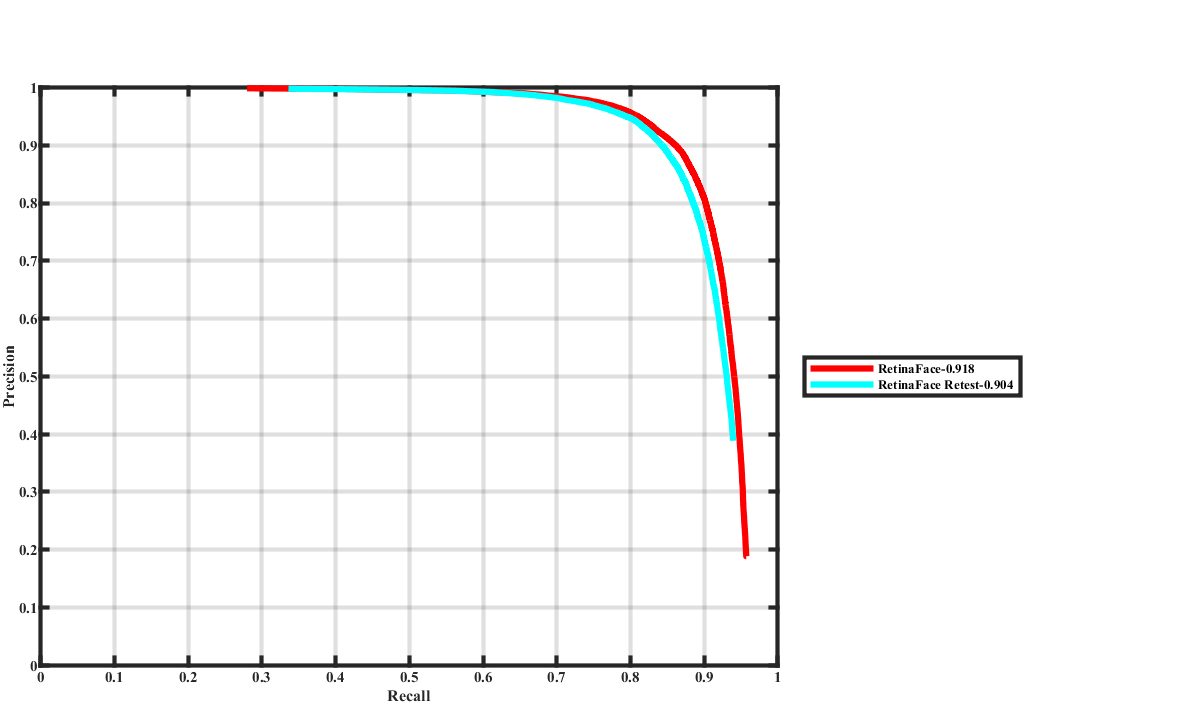
\includegraphics[width=0.75\linewidth]{wider_pr_cruve_int_hard_val.png}
		\caption{Hard Val}
	\end{figure}
	
\end{frame}
\begin{frame}
	\frametitle{New Data}
	\begin{itemize}
		\item Images are manually obtained and  we  want to recognize faces that are not part of any current dataset
		\item we need to gather examples of faces we want to recognize and then quantify them in some manner. This is done by facial recognition enrollment 
\item Another approach is that we  can programmatically download example images of the faces via APIs on varying platforms. Such as Bing’s image search API
\item Then we manually label them and annotate bounding boxes for localization of target face
		The out put file is in the form of text file with face bounding boxes and five facial landmark coordinates.
		\item Facial recognition datasets like MPII and Deepfake are available on open source platforms like Kaggle and could potentially be considered here.
	\end{itemize}
\end{frame}
\end{document}